\documentclass[dvipdfmx]{jsarticle}

\usepackage[version=3]{mhchem}
\usepackage{amsmath}
\usepackage[siunitx]{circuitikz}
\usepackage{graphicx}
\usepackage{here}

\setlength\parindent{0pt}

\begin{document}
\title{情報通信工学レポート}
\author{工学部電子情報工学科3年 03190449  堀 紡希}
\date{\ 10月16日}
\maketitle

\section*{レポート課題1}

\begin{enumerate}
\item[(a)]
\begin{align*}
s(t) &= \left(1+m(t)\right)\cdot c(t)\\
&= A_{c}\left(1+a\cos{(2\pi f_{m}t)}\right)\cos{(2\pi f_{c}t)}\\
&= A_{c}\cos{(2\pi f_{c}t)} + A_{c}a\cos{(2\pi (f_{c}+f_{m})t)} + A_{c}a\cos{(2\pi (f_{c}-f_{m})t)}
\end{align*}
より、スペクトルは以下の図

\begin{center}
\begin{figure}[H]
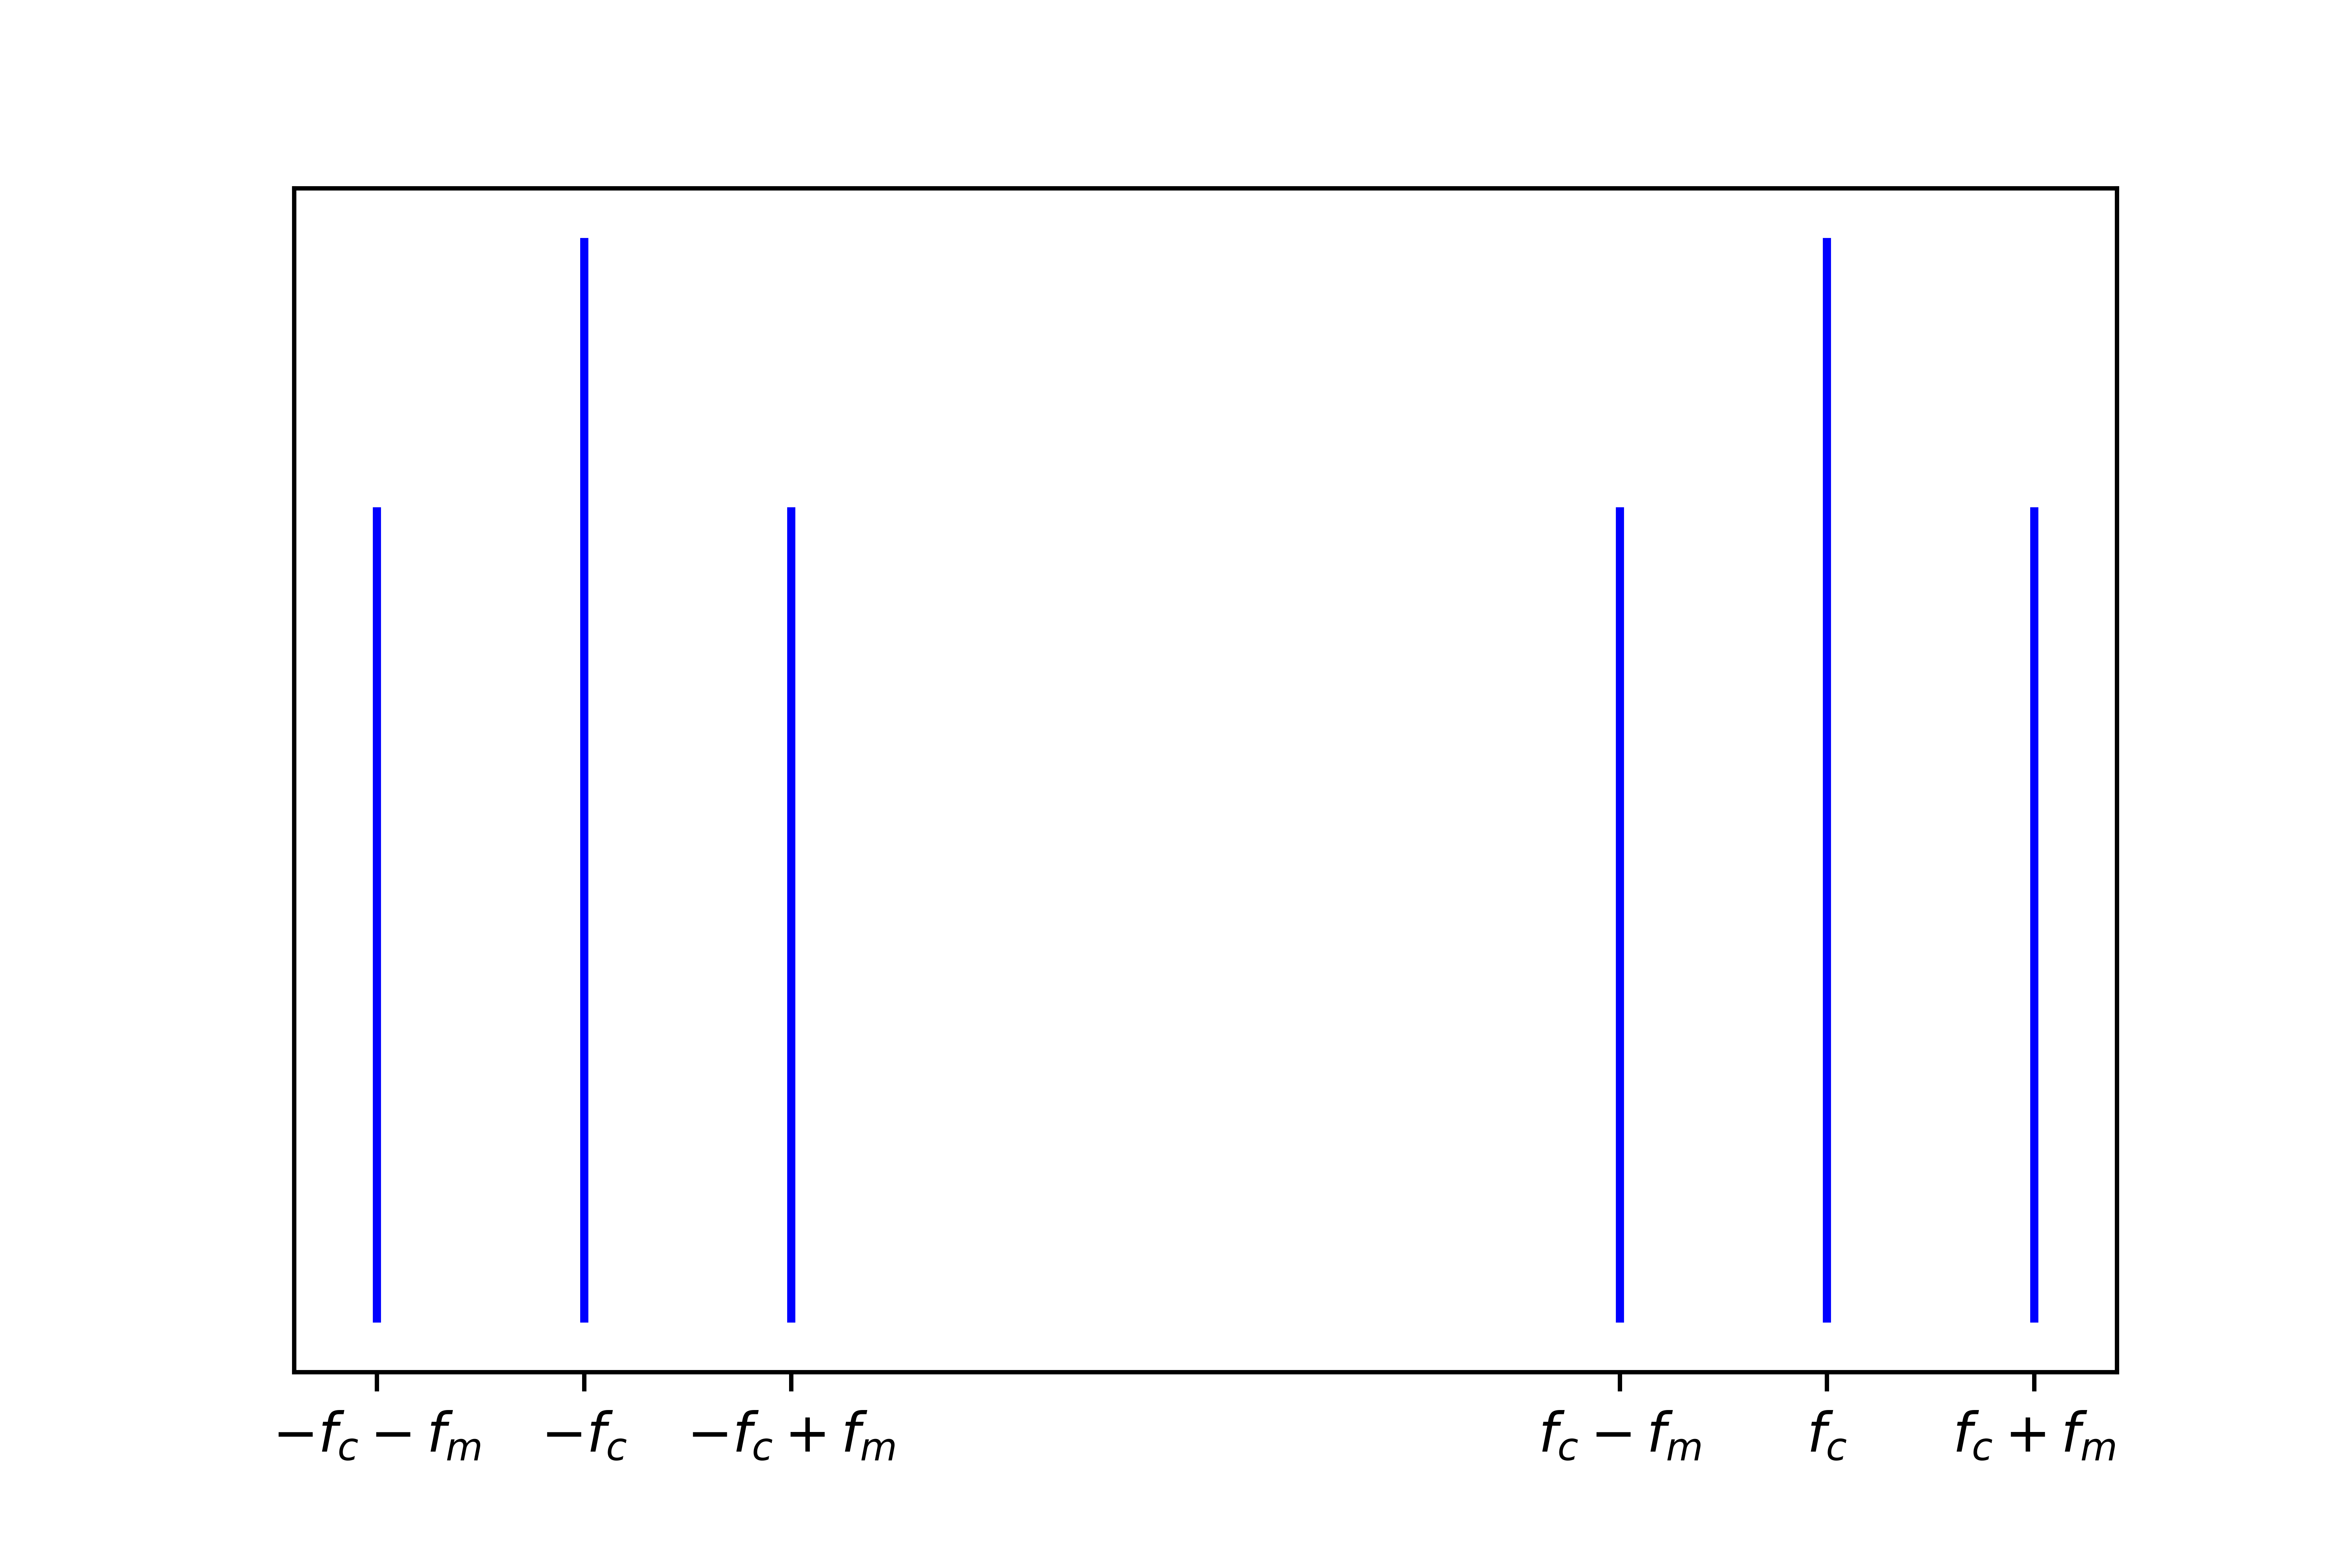
\includegraphics[scale = 1]{3_1.png}
\caption{1.(a)のスペクトル}
\end{figure}
\end{center}

\item[(b)]
信号
\begin{align*}
x_{1}(t) &= c(t) + m(t)\\
x_{2}(t) &= c(t) - m(t)
\end{align*}
を生成し、$y$で非線形変換し、差を取ると、
\begin{align*}
y_{1}(t) - y_{2}(t) &= \alpha x_{1}(t) + \beta x_{1}^{2}(t) - \alpha x_{2}(t) + \beta x_{2}^{2}(t)\\
&= 2\alpha m(t) + 4\beta m(t)c(t)\\
&= 2\alpha a\cos{(2\pi f_{m}t)} + 4\beta a\cos{(2\pi f_{m}t)}\cdot A_{c}\cos{(2\pi f_{c}t)}
\end{align*}
これを$\pm f_{c}$を通すバンドパスフィルタを通すと,$f_{c}>>f_{m}$より第一項が除去される。

この信号に$4\beta c(t)$を足し合わせると、
\begin{align*}
4\beta a\cos{(2\pi f_{m}t)}\cdot A_{c}\cos{(2\pi f_{c}t)} + 4\beta c(t) &= 4\beta m(t)c(t) + 4\beta c(t) \\
&= 4\beta\left(1+m(t)\right)c(t)
\end{align*}
となって、AM変調信号が得られる。
\end{enumerate}
\section*{レポート課題2}
\begin{enumerate}
\item[(a)]
出力信号$y(t)$は、
\begin{align*}
y(t) &= \left(\cos{(2\pi f_{m}t)} + \cos{(2\pi f_{c}t)}\right)^{2} \\
&= \cos{(2\pi f_{m}t)}^{2} + \cos{(2\pi f_{c}t)}^{2} + 2\cos{(2\pi f_{m}t)} \cos{(2\pi f_{c}t)}\\
&= 1+\frac{1}{2} \cos{(2\pi \cdot2f_{m}t)} + \frac{1}{2}\cos{(2\pi \cdot 2f_{c}t)} + \cos{(2\pi (f_{c}+f_{m})t)} + \cos{(2\pi (f_{c} -f_{m})t)}
\end{align*}
スペクトルは以下のようになる。

\begin{center}
\begin{figure}[H]
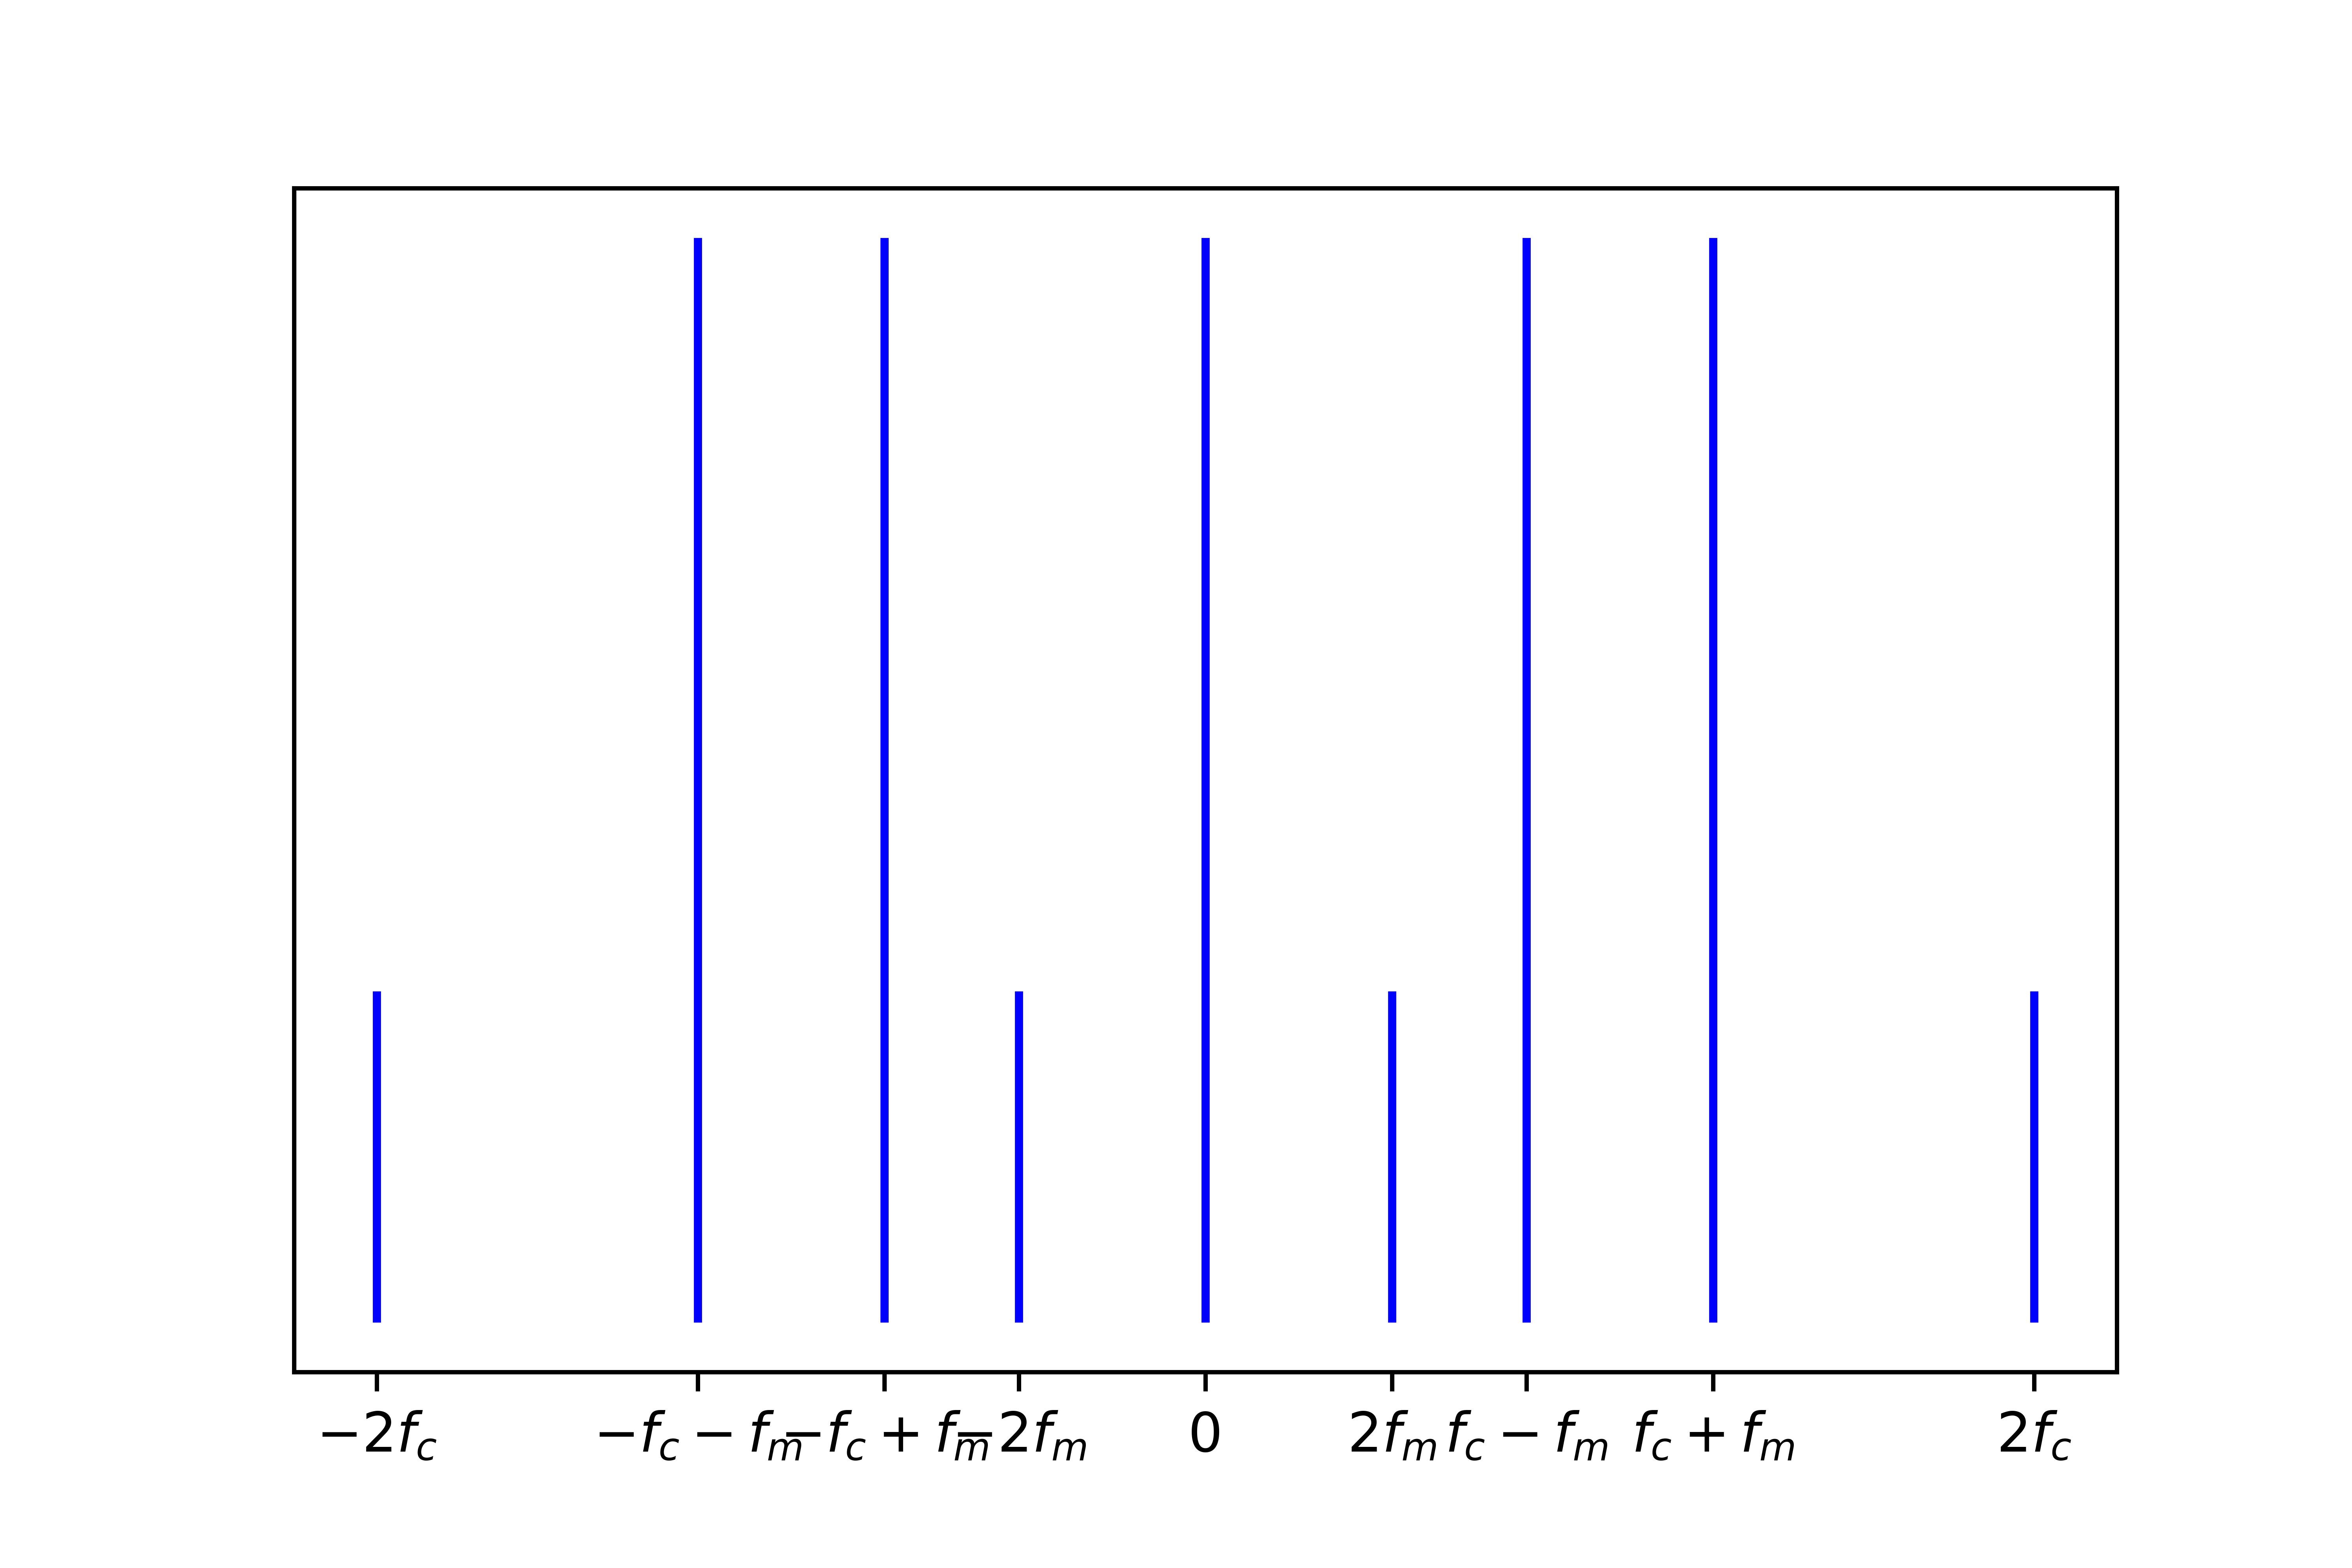
\includegraphics[scale = 0.8]{3_2.png}
\caption{2.(a)のスペクトル}
\end{figure}
\end{center}

\item[(b)]
$f_{c}$の周辺のスペクトルが得られれば良いので、
\[ 2f_{m} < f_{c} - f_{0} < f_{c} - f_{m}\]
と
\[f_{c}+f_{m} < f_{c} + f_{0} < 2f_{c}\]
を満たせば良いので、求める条件は、
\[f_{m} < f_{0} < f_{c} - 2f_{m}\]


\item[(c)]
周波数が$\Delta f$ずれたとき、
復調した信号は、
\[
m(t)\cdot \cos{(2\pi f_{c}t)}\cdot \cos{(2\pi (f_{c}+\Delta f)t)} = m(t)\cdot \frac{1}{2} \left(\cos{(2\pi(2f_{c}+\Delta f)t)}+\cos{(2\pi\Delta ft)}\right)
\]
となり、$\phi$が十分小さいとすると$\cos{\phi}$倍小さくなる。
位相が$\phi$ずれたとき、
復調した信号は、
\[
m(t)\cdot \cos{(2\pi f_{c}t)}\cdot \cos{(2\pi f_{c}t+\phi)} = m(t)\cdot \frac{1}{2} \left(\cos{(4\pi f_{c}t+\phi)}+\cos{\phi}\right)
\]
となり、$\phi$が大きくなるほど、復調信号の振幅が小さくなっていく。
\end{enumerate}



\section*{レポート課題3}
\begin{enumerate}
\item[(a)]
$S_{USB}(t) = m(t)\cos{(2\pi f_{c}t)} - m_{h}(t)\sin{2\pi f_{c}t}$
を、$\cos{(2\pi (f_{c}+\Delta f)t + \phi)}$で復調して、
\begin{align*}
&S_{USB}\cdot \cos{(2\pi (f_{c}+\Delta f)t + \phi)} \\
=&m(t)\frac{1}{2}\cdot \left(\cos{(2\pi (2f_{c}+\Delta f)t+\phi)} + \cos{(2\pi \Delta ft+\phi)} \right) - m_{h}(t)\frac{1}{2}\cdot \left(\sin{(2\pi (2f_{c}+\Delta f)t+\phi)} - \sin{(2\pi \Delta ft+\phi)} \right)
\end{align*}
\item[(b)]
$m(t) = \cos{(2\pi f_{m} t)}$として、(a)の式に代入すると、
\begin{align*}
S_{USB}(t) = &\frac{1}{4}\left(\cos{\left(2\pi(2f_{c}+f_{m}+\Delta f)t+\phi\right)}+\cos{\left(2\pi(\Delta f-f_{m})t+\phi\right)}\right) (t>0)\\
&\frac{1}{4}\left(\cos{\left(2\pi(2f_{c}-f_{m}+\Delta f)t+\phi\right)}+\cos{\left(2\pi(\Delta f+f_{m})t+\phi\right)}\right) (t<0)
\end{align*}

一方、2.(c)に$m(t)$を代入すると、
\begin{align*}
\frac{1}{4}\{\cos{(2\pi(2f_{c}+f_{m}+\Delta f)t+\phi)}+\cos{(2\pi (2f_{c}-f_{m}+\Delta f)t+\phi)}+\cos{(2\pi(f_{m}+\Delta f)t)} + \cos{(2\pi (f_{m}-\Delta f)t)}\}
\end{align*}
となり、第二項、第三項によりSSBによって得られた変調信号にさらに誤差が加わる形となっている。

つまり、SSB変調信号の方が復調用搬送波の誤差に対して強いと言える。

\end{enumerate}
\end{document}










